\documentclass{beamer}

\input{../preambulo/inputenc.tex}
\input{../preambulo/fuente.tex}
\input{../preambulo/spanish.tex}
\input{../preambulo/tikz.tex}
\input{../preambulo/matematica.tex}
\input{../preambulo/colors.tex}
\input{../preambulo/flotantes.tex}
\input{../preambulo/beamer_zub.tex}
\input{../preambulo/paquetes.tex}
\usepackage{ccicons}
% \ccPublicDomain

\newcommand{\etal}{{\it et al.}}
\newcommand{\ie}{{\it i. e.}}
\newcommand{\zlink}[1]{\href{#1}{\color{celeste}\faExternalLink*}}


\graphicspath{{../img/}{img/}}
\framebg{bg/pizarron3.png} 
\hypersetup{colorlinks=true, urlcolor=azul!40!white}

\begin{document}

\newcommand\CC{}

\begin{zframe}{}% yscale=0.9, % with frametitle
\path(cp) ++(3,0) node(I)[]{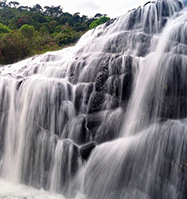
\includegraphics[width=6cm]{bakersfall2.jpg}};
\path(c2|-I.north) ++(0,-.5) node(A)[anchor=north,align=left]{
  \color{verde} \large\textbf{Métodos Computacionales}\\[3mm]  
  \color{celeste} \textbf{Dinámica Molecular}\\[2mm]  
  \color{lila} \textit{Octubre 29, 2025}
};
\normalsize
\path(A.west|-I.south) ++(0,.5) node(B)[anchor=south west,align=left]{
  S. Alexis Paz\\[5mm]

\includegraphics[width=3cm]{logos/DQTC_orange.png}};

\path(I.south east) ++(0,0) node[anchor=north east,inner sep=0]{
  \href{https://www.gorgeouslanka.com/horton-plains}{\tiny Horton Plains}}; 
 
\end{zframe}

\renewcommand\CC{
  \path(se) node[anchor=south east]{\tiny\color{gray} MC2025 - S.A.Paz};}
           
\begin{zframe}{
  titulo/.style={verde, align=center},
  texto/.style={anchor=north,align=left}
}

\large

\path(cp|-t) ++(0,.3) node(T)[titulo]{
\LARGE Dinámica};

\path(cp|-T.south) ++(0,0) node(T)[texto]{
Estudia el movimiento en relación con {\color{naranja}las causas que lo
  producen}.
};
 
\path(cp|-T.south) ++(0,-.1) node(T)[texto]{
  {\Large \color{verde} Ecuaciones de movimiento}, \textit{por ejemplo\ldots}:
};
  
\path(t|-T.south) ++(-.4,-.2) node(T)[texto,anchor=north west]{
\color{celeste}Newton\\[2mm]
$\ds m\odv[order=2]{\vb{r}}{t}=-\nabla U(\vb{r})$
};

% La ecuacion de Fokker Plank describe la evolucion de densidades de probabilidad.
% En equilibrio, genera la distribución de Boltzman.

% La ecuacion de probabilidad de Fokker plank con difusion constante y sin
% drift describe las probabilidades del movimiento browniano. 

% La ecuacion de Langevin describe el movimiento de las particulas en el
% movimiento Browniano. La ecucacion de Langevin genera una forma particular
% de la de Fokker Planck.

% La ecuacion de movimiento Browniana clasica, o sobreamortiguada, es la de
% lagnevin sobre amortiguada, i.e. acelearcion promedio cero. Esta genera una
% ecuacion de Fokker Planck particular que se conoce como ecuacion de
% Smoluchowski.

% The Fokker–Planck equation for an underdamped Brownian particle is called
% the Klein–Kramers equation. NOTA: entiendo que underdamped Brownian
% es directamente la de langevin

% El commitor es la solucion de la ecuacion de cierta Fokker Plank
% independiente del tiempo en el espacio de los estados. \cite{ciccotti_2015}

 
\path(t|-T.south) ++(-.4,-.3) node[texto,anchor=north west]{
\color{celeste}Barostato de Andersen\\[2mm]
${\ds\odv{\vb{r}}{t} = \dfrac{\vb{p}}{m}+\frac{\vb{r}}{3}\odv{\ln V}{t}}$\\[2mm]
${\ds\odv{\vb{p}}{t} = -\nabla U-\frac{\vb{p}}{3}\odv{\ln V}{t}}$\\[2mm]
${\ds\odv[order=2]{V}{t}=\dfrac{p_0}{M}+\dfrac{\ab(\vb{p}^2/m-\nabla U)}{3MV}}$
};
 
    
\path(cp|-T.east) ++(-1.9,.3) node(T)[texto,anchor=west]{
{\color{celeste}Langevin}
${\ds m \pdv{\vb{v}}{t}=-\nabla U-\gamma \vb{v}+\sqrt{2\gamma k_BT}\boldsymbol\eta }$\\[2mm]
};
                  
\path(cp|-T.south) ++(-2,.3) node(T)[texto,anchor=north west]{
{\color{celeste}Browniano}
${\gamma \vb{v}=-\nabla U+\sqrt{2\gamma k_BT}\boldsymbol\eta }$\\[2mm]
};
                  
\path(cp|-T.south) ++(0,.2) node(T)[texto,anchor=north west]{
\color{celeste}DM acelerada por temperatura\\[2mm]
${\ds\gamma \odv{\vb{r}}{t}= -\nabla U+\sqrt{2\gamma k_BT}}$\\[2mm]
${\ds\quad\quad-\kappa\ab({\boldsymbol \theta}-\vb{z})\nabla \vb{\boldsymbol\theta}\boldsymbol\eta^x}$\\[2mm]
${\ds\bar{\gamma}\odv{\vb{z}}{t}= \kappa\ab({\boldsymbol\theta}-\vb{z})+\sqrt{2\bar{\gamma}k_B\bar{T}}\boldsymbol\eta^z}$\\[2mm]
};

\end{zframe}
  
\begin{zframe}{yscale=0.9}
\frametitle{Dinámica Molecular}

                      
\path(c2) ++(.5,0) node(A){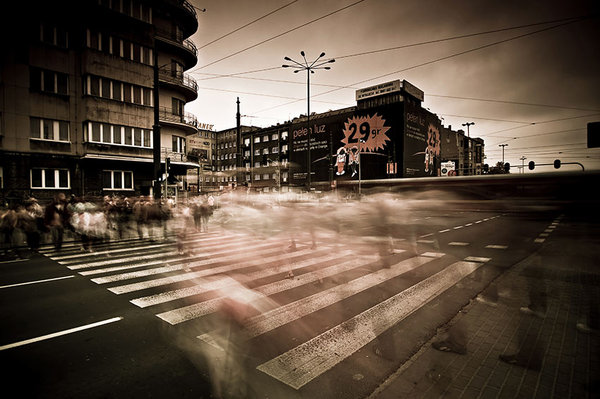
\includegraphics[width=6cm]{peopole_longexp.png}};
\path(A.south west) ++(0.,.2) node[anchor=north west]{\tiny ``Rush'', \href{hhttps://www.behance.net/gallery/346775/Rush/modules/174420}{Tomasz 'Darkshape' Kaluzny}}; 
% Esta foto es CC BY-NC-ND

\path(c3) ++(.5,0) node(A){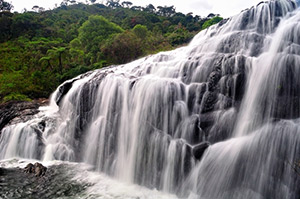
\includegraphics[width=6cm]{bakersfall.jpg}};
\path(A.south west) ++(0.,.2) node[anchor=north west]{\href{https://www.gorgeouslanka.com/horton-plains}{\tiny Horton Plains}}; 

\path(cp) ++(.8,.3) node(A){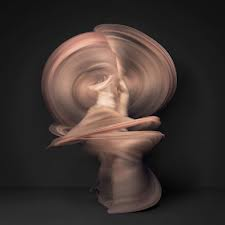
\includegraphics[width=3.5cm]{bailarinalongexp.jpeg}};
\path(A.south east) ++(-.2,.2) node[anchor=north east,align=right]{\tiny ``nude'' \\[-2mm] \tiny\href{https://www.shinichimaruyama.com/works/}{Shinichi Maruyama}}; 
                                       
\path(c1) ++(0,0) node(A){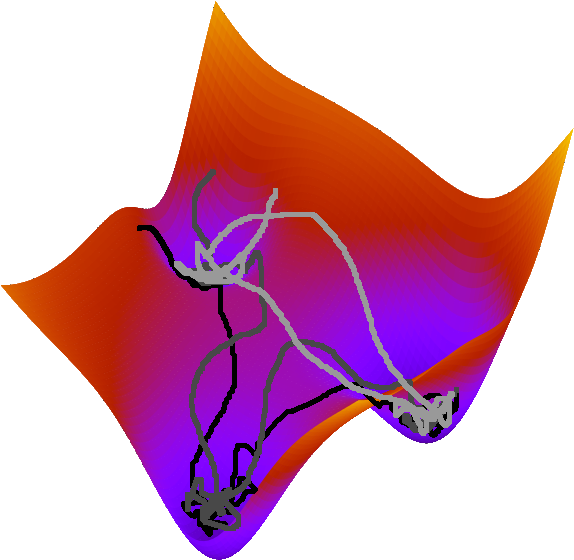
\includegraphics[width=4cm]{SEP_raya33.png}};
\path(c4) ++(0,0) node(A){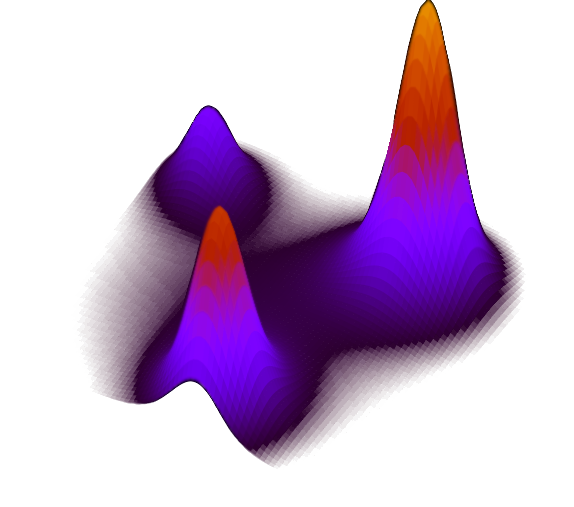
\includegraphics[width=4cm]{DOS.png}};
                    
\end{zframe}
       
\begin{zframe}{yscale=0.9}
\frametitle{Densidad de Probabilidad en el Espacio de las Fases} 

\node[zf/title=center]{$\rho(\vb{q},\vb{p},t)$};

\node[zf/text=return]{Newton -> Ecuación de Liouville};
\node[zf/text=right]{En equilibrio \color{amarillo}$\ds\rho(\vb{q},\vb{p})=\Omega^{-1}$};

\node[zf/text=return]{Langevin -> Ecuación de Fokker Planck};
\node[zf/text=right]{En equilibrio \color{amarillo}$\ds\rho(\vb{q},\vb{p})=\Z^{-1}e^{\beta H(\vb{q},\vb{p})}$};
\path(c3) ++(.2,2.8) node[celeste]{\small (integrales estocásticas)};

\path(vl) ++(0,-.5) node(A){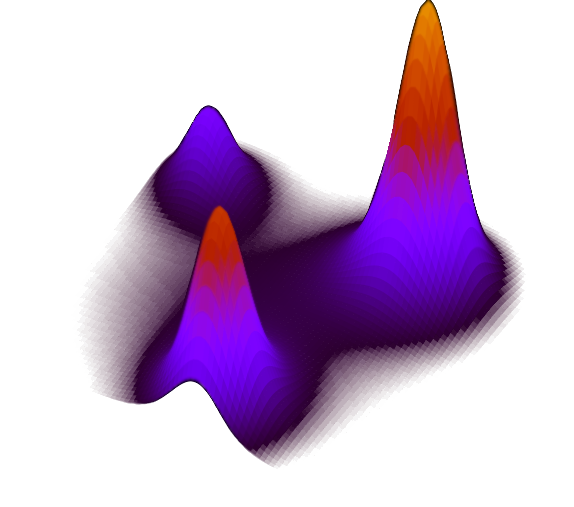
\includegraphics[width=4cm]{DOS.png}};

% \node[zf/text=next]{$\odv{\rho}{t}=\pdv{\rho}{t}+\pdv{\rho}{\vb{q}}\odv{\vb{q}}{t}+\pdv{\rho}{\vb{p}}\odv{\vb{p}}{t}=0$};
% Liouville asegura que si empiezas con esta distribución uniforme, permanece uniforme
% La hipótesis fundamental selecciona la distribución uniforme como la de equilibrio
%
\end{zframe}
       
\begin{zframe}{
  titulo/.style={verde, align=center},
  texto/.style={anchor=north,align=left}
}

\large

\path(cp|-t) ++(0,.2) node(T)[titulo]{
\LARGE Distribución de equilibrio};

\path(cp|-T.south) ++(0,-.1) node(T)[texto]{
¿Qué probabilidad de encontrar un estado del sistema generan?
};
 
 
\path(t|-T.south) ++(-.4,-.75) node(T)[texto,anchor=north west]{
\color{celeste}Newton\\[2mm]
$\ds\rho(\vb{r})=\Omega^{-1}$, \ $NVE$
};

% La ecuacion de Fokker Plank describe la evolucion de densidades de probabilidad.
% En equilibrio, genera la distribución de Boltzman.

% La ecuacion de probabilidad de Fokker plank con difusion constante y sin
% drift describe las probabilidades del movimiento browniano. 

% La ecuacion de Langevin describe el movimiento de las particulas en el
% movimiento Browniano. La ecucacion de Langevin genera una forma particular
% de la de Fokker Planck.

% La ecuacion de movimiento Browniana clasica, o sobreamortiguada, es la de
% lagnevin sobre amortiguada, i.e. acelearcion promedio cero. Esta genera una
% ecuacion de Fokker Planck particular que se conoce como ecuacion de
% Smoluchowski.

% The Fokker–Planck equation for an underdamped Brownian particle is called
% the Klein–Kramers equation. NOTA: entiendo que underdamped Brownian
% es directamente la de langevin

% El commitor es la solucion de la ecuacion de cierta Fokker Plank
% independiente del tiempo en el espacio de los estados. \cite{ciccotti_2015}


% https://arxiv.org/pdf/2111.06402
% A Fully Anisotropic Formulation of Stochastic Cell Rescaling
% Aqui explica que el ensamble de Andersen es isoenthalpic-isobaric NPH que
% temrina siendo NPT para grandes grados de libertad.
 
\path(t|-T.south) ++(-.4,-.63) node[texto,anchor=north west]{
\color{celeste}Barostato de Andersen\\[2mm]
$\ds\rho(\vb{r})=Z^{-1}e^{\beta U(\vb{r})+\beta PV}$\\[2mm]
$NPH\to NPT$
};

% Advanced molecular dynamics techniques ChE210D
% Today's lecture: how to perform molecular dynamics at constant temperature, for
% systems with rigid bonds, and for systems with multiple time scales 

% In the limit of an infinitely long trajectory averaged over many heat bath collisions, it can be
% shown that the Andersen thermostat rigorously generates the correct canonical ensemble probabilities. That is, the distribution of kinetic and potential energies, and the microstate probabilities of different configurations of the system, all rigorously approach their true form in the canonical ensemble.
% However, the presence of random collisions causes the velocities of particles to decorrelate
% (“lose memory” of their initial values from some previous point in time) much faster than the
% NVE dynamics. As a result, true molecular kinetics are not preserved by the Andersen thermostat. For example, the computed diffusion constants for particles would give erroneous values

% En cambio, nose-hover
% The implication of this result is that a microcanonical simulation in the
% extended system (including heat bath degrees of freedom) returns a
% canonical ensemble for the original system. That is, if we evolve the
% extended system according to the extended Hamiltonian above (more exactly,
    % the extended underlying Lagrangian), we expect to obtain a canonical
% distribution of the particle positions and momenta. This evolution will
% correspond to solving the trajectory for the atomic coordinates and momenta
% as well as the heat bath degrees of freedom 𝑠 and 𝑝𝑠.  Importantly, this
% thermostat rigorously generates canonical ensemble thermodynamics and can
% approximate the true dynamics of the system because the time evolution of
% the particles is deterministic, and doesn’t involve stochastic changes. 
    
\path(cp|-T.east) ++(-1.8,.4) node(T)[texto,anchor=west]{
{\color{celeste}Langevin}
$\ds\rho(\vb{r})=Z^{-1}e^{\beta U(\vb{r})}$,\  $NVT$
};
                  
\path(cp|-T.south) ++(-1.8,-.3) node(T)[texto,anchor=north west]{
{\color{celeste}Browniano}
$\ds\rho(\vb{r})=Z^{-1}e^{\beta U(\vb{r})}$,\  $NVT$
};
                  
\path(cp|-T.south) ++(0,-.4) node(T)[texto,anchor=north west]{
\color{celeste}DM acelerada por temperatura\\[2mm]
$\ds\rho(\vb{r})=Z^{-1}e^{\beta \ab(U(\vb{r})+\kappa\ab({\boldsymbol\theta}-\vb{z})^2/2)}$\\[2mm]
$\ds\rho(\vb{z})\approx\bar{Z}^{-1}e^{\bar\beta F(\vb{z})}$
};
            
\path(sp) ++(0,.2) node(T)[texto,anchor=south]{
\color{naranja} \it ¡Pero la dinámica también muestrea fuera del equilibrio!\\[2mm]
};
        
\end{zframe}
   
     
        
\begin{zframe}{yscale=0.9}
\frametitle{Ecuación de Newton} 

\path(ne) +(-1,0.5) node[align=center,rectangle,red,draw,fill=white,text width=5cm,rotate=-30, ultra thick]{\bfseries ``REPASO''};

\path(ne) ++(-.3,-.3) node(T)[align=left,anchor=north east]{
  {\Large \color{celeste}$\ds\odv[order=2]{y}{x}=G(x,y)$} };
                       
\path(t) node[title]{Verlet};
                       
\path(t|-title.south) ++(0,-.5) node(T)[align=left,anchor=north west,text width=6cm]{
  ${\ds y_{n+1}=2y_{n}-y_{n-1}+G(x_n,y_n)h^2+O\ab(h^4)}$ };
  
\path(vl) ++(0,-1) coordinate(scope);
\begin{scope}[x=1cm,y=1cm,scale=1.5,shift=(scope),thick,yrange=-1:3]
  \newcommand\xmin{-2}
  \newcommand\xmax{2}
  \newcommand\xstp{1}
  \newcommand\xtra{1}
  \newcommand\ymin{0.5}
  \newcommand\yorg{0.5}
  \newcommand\ymax{3}
  \newcommand\ystp{1}
  \newcommand\nfra{1}

  { \input{frames/euler.tex}}
 
  \pgfmathsetmacro\xo{-1}
  \pgfmathsetmacro\x{0}
  \pgfmathsetmacro\ox{1}
  \pgfmathsetmacro\yo{sin((\xo-(\xtra))/3.1415*180)+2}
  \pgfmathsetmacro\y{sin((-(\xtra))/3.1415*180)+2}
  \pgfmathsetmacro\oy{sin((\ox-(\xtra))/3.1415*180)+2}

  \draw[celeste, dashed, ultra thick, domain=\xmin:\xmax] plot[smooth,id=parabola] 
  function{\yo*(x-\x)*(x-\ox)/2-\y*(x-\xo)*(x-\ox)+\oy*(x-\xo)*(x-\x)/2};
                        
  
  % Pendiente
  \pgfmathsetmacro\y{sin((-(\xtra))/3.1415*180)+2}
  \pgfmathsetmacro\a{cos((0-(\xtra))/3.1415*180)}
               
  % yn+1
  \pgfmathsetmacro\xo{-1}
  \pgfmathsetmacro\yo{sin((\xo-(\xtra))/3.1415*180)+2}
  \draw[color=celeste,domain=-1:1,ultra thick] plot[smooth] function{(\a*(x-\xo)+\yo)};
  \draw[celeste](\xo,\yo) circle(.1) node[fg,above=.1]{ $y_{n-1}$};
  \pgfmathsetmacro\oy{(\a*(1-\xo)+\yo)};
  \fill[naranja](1,\oy) circle(.1) node[fg,above=.1]{ $y_{n+1}$};
 
  % yn-1
  \fill[celeste](0,\y) circle(.1) node[fg,below=.1]{ $y_{n}$};
  \pgfmathsetmacro\y{sin((-1-(\xtra))/3.1415*180)+2}
   
\end{scope}
          
\end{zframe}
      
\begin{zframe}{yscale=0.9}
\frametitle{Ecuación de Newton} 

\path(ne) ++(-.3,-.3) node(T)[align=left,anchor=north east]{
  {\Large \color{celeste}$\ds m\odv[order=2]{\vb{r}}{t}=\vb{F}=-\nabla U(\vb{r})$}; };
                       
\path(t) node[title]{Verlet};
                       
\path(t|-title.south) ++(0,-.5) node(T)[align=left,anchor=north west,text width=6cm]{
  ${\ds \vb{r}_{n+1}=2\vb{r}_{n}-\vb{r}_{n-1}+\dfrac{h^2}{m}\vb{F}_n+O\ab(h^4)}$ };
  
\only<1,2>{

\path[verde] (c4)  circle(.1)  coordinate(O);
\path(cp) ++(0,-1) ++(-120:2) coordinate(A);
\path(cp) ++(0,-1) coordinate(B);
\path<1>(cp) ++(0,-1) ++(90:1.5) coordinate(C);
\path<2>(cp) ++(0,-1) ++(60:2) coordinate(C);


\path(O) node[fg,below=.1,verde]{ origen };
\path(A) node[fg,below=.1]{ $\vb{r}_{n-1}$};
\path(B) node[fg,right=.1]{ $\vb{r}_{n}$};
\path(C) node[fg,left=.1]{ $\vb{r}_{n+1}$};

\draw[verde,dashed,ultra thick,->] (O) -- (B);
\draw[celeste,ultra thick,->] (A) -- (B) node[pos=0.5,left]{$\vb{r}_{n}-\vb{r}_{n-1}$};
\draw<1>[celeste,ultra thick,->] (B) -- (C);
\draw<2>[celeste,ultra thick,->] (B) -- (C) node[pos=0.5,left]{$\vb{r}_{n+1}-\vb{r}_{n}$};
\draw<1>[amarillo,ultra thick,->] (B) -- ++(160:1) node[pos=1,left]{$\vb{F}_n$};


\draw[verde](O) circle(.1);
\draw[celeste](A) circle(.1);
\fill[celeste](B) circle(.1);
\fill[naranja](C) circle(.1);
 
}


\path[verde]<3>(t|-cp) ++(0,0) node(T)[title]{\Large Velocity Verlet:};
                                

\path<3>(t|-title.south) ++(0,-.1) node(T)[align=left,anchor=north west]{
${\ds{\vb{r}_{n+1} = \vb{r}_{n} + \vb{v}_{n}\Delta t + \frac{\vb{F}_{n}}{2m}  \Delta t^2}+O\ab(h^3)}$\\[2mm] 
${\ds \vb{v}_{n+1} = \vb{v}_n + \frac{\vb{F}_n+{\color{celeste}\vb{F}_{n+1}}}{2m} \Delta t+O\ab(h^3)}$ };
          
\end{zframe}
      
 
\begin{zframe}{yscale=0.9}
\frametitle{Movimiento Browniano y/o Ecuacion de Langevin} 
                 
\path(t) ++(-.3,-1.3) node[title]{ Browniano Convencional};
                       
\path(ne) ++(-.3,-.3) node[align=left,anchor=north east]{
  {\Large \color{celeste}${\ds\frac{dx(t)}{dt} = \sqrt{2D}\, \eta(t)
 \quad\langle \eta(t) \rangle = 0, 
 \;
 \langle \eta(t)\eta(t') \rangle = \delta(t - t')}$}};
 
\path(t|-title.south) ++(-.4,-.1) node(T)[align=left,anchor=north west]{
${\ds \vb{r}_{n+1} = \vb{r}_{n} + \dfrac{\Delta t}{m\gamma}F_n+\sigma_X\vb{X}_G}\quad\quad \sigma_X=\sqrt{\dfrac{2k_BT\Delta t}{m\gamma}}$
};
         
            
\path(ep) ++(-.3,0.4) node[align=left,anchor=north east]{
  {\Large \color{celeste}${\ds m \frac{d^2 x(t)}{dt^2} = -\gamma \frac{dx(t)}{dt} + F(x,t) + \xi(t)}$}};
          
  
\path(t|-T.south) ++(-.3,-2) node[title]{\color{verde} \Large Ermak};
 
\path(t|-title.south) ++(-.4,-.1) node[align=left,anchor=north west]{
${\ds\vb{r}_{n+1}=\vb{r}_{n}+c_1\Delta t \vb{v}_{n}+c_2\Delta t^2 \frac{F_{n}}{m}+ \sigma_X\vb{X}_G}$\\[2mm]
${\ds\vb{v}_{n+1}=c_0 \vb{v}_{n}+c_1\Delta t \frac{F_{n}}{m}+\frac{c_2\Delta t}{m} \ab(F_{n+1}-F_{n})+\sigma_V\ab(\sigma_{V,X}\vb{X}_G+\sigma_{V,V}\vb{V}_G)}$
};
         

% \path(ep) ++(-.3,-2) node[align=left,anchor=north east]{
%   {\color{celeste}Langevin}
% };
                    
\end{zframe} 
      
\begin{zframe}{yscale=0.9}
\frametitle{Integracion de los momentos (NVT)}

\path(t) ++(-.2,-.2) node(T)[align=left,anchor=west]{
  {\color{celeste} Distribución de Maxwell-Boltzmann}\ \ / \color{naranja} \ \ Espacio de configuraciones
};

\path(t|-T.south) ++(1,-.2) node(T)[align=left,anchor=north west]{
  ${\ds\rho(\vb{p},\vb{r})=Z^{-1}e^{-\beta H(\vb{p},\vb{r})}}$\\[2mm]
  ${\ds\quad\quad\quad={\color{celeste}\frac{e^{-\beta \vb{p}^2/2m}}{\int_{\vb{p}}e^{-\beta \vb{p}^2/2m}\odif{\vb{p}}}}\color{naranja}\frac{e^{-\beta U(\vb{r})}}{\int_{\vb{r}}e^{-\beta U\ab(\vb{r})}\odif{\vb{r}}}}$\\[2mm]
  ${\ds\quad\quad\quad={\color{celeste}\ab(\frac{\beta}{2m\pi})^{\frac{3}{2}}e^{-\beta \vb{p}^2/2m}}\color{naranja}\frac{e^{-\beta U(\vb{r})}}{Q}}$\\[2mm]
  ${\ds\quad\quad\quad={\color{celeste}\tilde f(\vb{p})}\color{naranja}q(\vb{r})}$ ${\ds\quad\quad\quad\tilde f(\vb{p})=f_1(p_x)f_1(p_y)f_1(p_z)}$
};
 
\path(t|-T.south) ++(1,-.2) node(T)[align=left,anchor=north west]{
  $\color{celeste}{\ds f(v)=\ab(\frac{m\beta}{2\pi})^{\frac{3}{2}}4\pi v^2 e^{-\beta mv^2/2}}\quad\color{naranja}{\ds \ab<A>=\int A(\vb{r})q(\vb{r})}\odif{\vb{r}}$
};
           
\end{zframe}
          
\begin{zframe}{yscale=0.9}
\frametitle{Otros Termostatos}
                  
\path(t) ++(-.4,.3) node(T)[align=left,anchor=north west]{
{\color{verde} \Large Berendsen:}
};
 
\path(t|-T.south) ++(-.4,.1) node(T)[align=left,anchor=north west,text width=10cm]{
$\vb{v}_{n+1} = \vb{v}_n\sqrt{1+\frac{\Delta t}{\tau}\left( \frac{T_0}{T} - 1 \right)}$
};
                 
\path(t|-T.south) ++(-.4,-.4) node(T)[align=left,anchor=north west]{
{\color{verde} \Large Andersen:}
};
    
\path(t|-T.south) ++(-.4,-.1) node(T)[align=left,anchor=north west]{
$\vb{v}_{n+1}=\sqrt{\frac{k_B T_0}{m_i}} \vb{X}_G \quad \text{con probabilidad } \nu \Delta t$
};
                

\path(t|-T.south) ++(-.4,-.4) node(T)[align=left,anchor=north west]{
{\color{verde} \Large Nosé-Hoover:}
};
 
\path(t|-T.south) ++(1.4,1.3) node(T)[align=left,anchor=north west,text width=10cm]{
\begin{align*}
\odv{\vb{r}_i}{t} &= \frac{\vb{p}_i}{m_i} \\
\odv{\vb{p}_i}{t} &= -\frac{\partial U}{\partial \vb{r}_i} - \zeta \vb{p}_i \\
\odv{\zeta}{t} &= \frac{1}{Q} \left( \sum_i \frac{\vb{p}_i^2}{m_i} - 3N k_B T_0 \right)
\end{align*}
};
         
 

          
\end{zframe}
          

                

\begin{zframe}{}
         
\path(t) ++(0,.5) node(T)[align=left,anchor=north west]{
{\color{verde} \Large Condiciones de Contorno \color{naranja} Periódicas}
};                                    


\path(hl) ++(-.3,.5) coordinate(media); 
\zfmedia[anchor=north east]{peli/mario.h264}{6cm}

\path(hr) ++(-.3,-1.5) coordinate(media); 
\zfmedia[anchor=north east]{peli/out_neg.h264}{7cm}
 
\end{zframe}

 
\begin{zframe}{}
          
\path(t) ++(0,.5) node(T)[align=left,anchor=north west]{
{\color{verde} \Large Condiciones de Contorno \color{naranja} Periódicas}
};                                    
  
\path(3,2) coordinate(scope);
\begin{scope}[x=1cm,y=1cm,amarillo,shift=(scope),thick]

% Definir
\path<1->(0,0) coordinate(O);
\path<1->(4,4) coordinate(K1);          % Esquina del cuadrante 1
\path<1->(K1-|{(0,4)}) coordinate(K2); % Esquina del cuadrante 2
\path<1->(K2|-{(0,0)}) coordinate(K3); % Esquina del cuadrante 3
\path<5>(-2,-2) coordinate(O);
\path<5>(9,5.8) coordinate(K1);          % Esquina del cuadrante 1
\path<5>(K1-|{(-1.8,5.8)}) coordinate(K2); % Esquina del cuadrante 2
\path<5>(K2|-{(-1.8,-1.8)}) coordinate(K3); % Esquina del cuadrante 3


% Emergentes
\path(K3-|K1) coordinate(K4);       % Esquina del cuadrante 4
\path(O-|K1) coordinate(xp);       % Punta de eje +x
\path(O-|K2) coordinate(xn);       % Punta de eje -x
\path(O|-K1) coordinate(yp);       % Punta de eje +y
\path(O|-K3) coordinate(yn);       % Punta de eje -y


% grid
\draw[ystep=4, xstep=4, ultra thick, celeste] (K3) grid (K1);

\fill(2,2)    circle(.1) coordinate(W);
\fill(1,.2)   circle(.1) coordinate(X);
\fill(3,3.8)  circle(.1) coordinate(Y);
\fill(3.6,.7) circle(.1) coordinate(Z);
\fill<5>(W) ++(0,-4) circle(.1) coordinate(W2);
\fill<5>(Y) ++(0,-4) circle(.1) coordinate(Y2);
\fill<5>(X) ++(0,4) circle(.1) coordinate(X2);
\fill<5>(Z) ++(0,4) circle(.1) coordinate(Z2);

\begin{scope}[ultra thick]
 
\clip<3>(0.1,0.1) rectangle ++(4,4);
\draw<2->[thick](Z) -- ++(200:1) coordinate(ZZ);
\draw<2->[->,thick](Z) -- ++(20:1) coordinate(ZZZ);
\draw<2->(Z)             node[above]{$\vb{r}_{n}$};
\draw<2->(ZZ) circle(.1) node[above]{$\vb{r}_{n-1}$};
\path<2->(ZZZ)           node[above]{$\vb{r}_{n+1}$};
                                  
\path<3->(Z) ++(-4,0) circle(.1) coordinate(Z);
\draw<3->[thick](Z) -- ++(200:1) coordinate(ZZ);
\draw<3->[->,thick](Z) -- ++(20:1) coordinate(ZZZ);
\draw<3->(Z)  circle(.1) node[above]{$\vb{r}_{n}$};
\draw<3->(ZZ) circle(.1) node[above]{$\vb{r}_{n-1}$};
\path<3->(ZZZ)           node[above]{$\vb{r}_{n+1}$};
\end{scope}
 
\fill<5>(W) ++(4,0) circle(.1) coordinate(W);
\fill<5>(X) ++(4,0) circle(.1) coordinate(X);
\fill<5>(Y) ++(4,0) circle(.1) coordinate(Y);
\fill<5>(Z) ++(4,0) circle(.1) coordinate(Z);
\fill<5>(W) ++(0,-4) circle(.1) coordinate(W2);
\fill<5>(Y) ++(0,-4) circle(.1) coordinate(Y2);
\fill<5>(X) ++(0,4) circle(.1) coordinate(X2);
\fill<5>(Z) ++(0,4) circle(.1) coordinate(Z2);

\fill<5>(W) ++(4,0) circle(.1) coordinate(W);
\fill<5>(X) ++(4,0) circle(.1) coordinate(X);
\fill<5>(Y) ++(4,0) circle(.1) coordinate(Y);
\fill<5>(Z) ++(4,0) circle(.1) coordinate(Z);
\fill<5>(W) ++(0,-4) circle(.1) coordinate(W2);
\fill<5>(Y) ++(0,-4) circle(.1) coordinate(Y2);
\fill<5>(X) ++(0,4) circle(.1) coordinate(X2);
\fill<5>(Z) ++(0,4) circle(.1) coordinate(Z2);

\fill<5>(W) ++(-12,0) circle(.1) coordinate(W);
\fill<5>(X) ++(-12,0) circle(.1) coordinate(X);
\fill<5>(Y) ++(-12,0) circle(.1) coordinate(Y);
\fill<5>(Z) ++(-12,0) circle(.1) coordinate(Z);
\fill<5>(W) ++(0,-4) circle(.1) coordinate(W2);
\fill<5>(Y) ++(0,-4) circle(.1) coordinate(Y2);
\fill<5>(X) ++(0,4) circle(.1) coordinate(X2);
\fill<5>(Z) ++(0,4) circle(.1) coordinate(Z2);
           
\end{scope} 
      

\end{zframe}
           
\begin{zframe}{}
         
\path(t) ++(0,.5) node(T)[align=left,anchor=north west]{
{\color{verde} \Large Condiciones de Contorno \color{naranja} Paredes Duras}
};                                    
  
\path(hl) ++(0,-.5) coordinate(media); 
\zfmedia[anchor=north east]{peli/arkanoid.h264}{7cm}

\path(hr) ++(-.2,-1.5) node(A){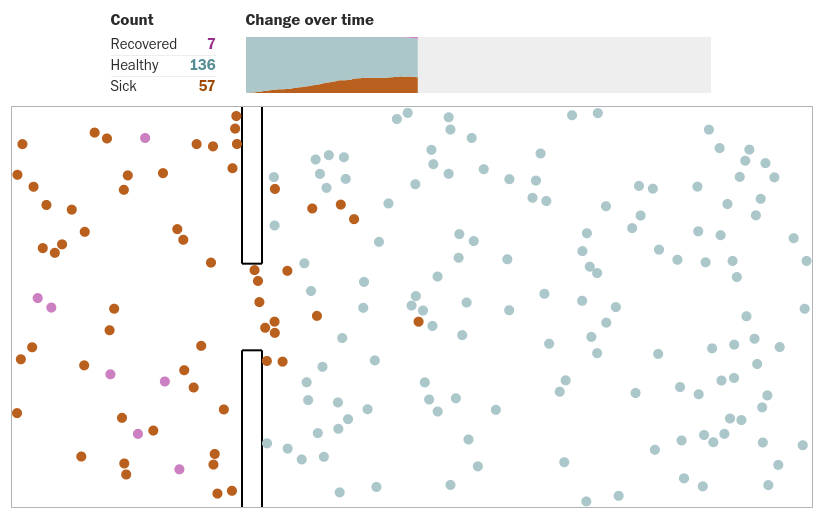
\includegraphics[width=7.5cm]{img/flaten.png}};
\path(A.south west) ++(0,0) node[anchor=north west,inner sep=0]{
  \tiny Stevens, \href{https://www.washingtonpost.com/graphics/2020/world/corona-simulator/}{The Washington Post, March 14, 2020}};
 
 
\end{zframe}
         
 
\begin{zframe}{}
         
\path(t) ++(0,.5) node(T)[align=left,anchor=north west]{
{\color{verde} \Large Condiciones de Contorno \color{naranja} Reservorios}
};                                    
  
\path(hl) ++(-.1,.5) coordinate(media); 
\zfmedia[anchor=north east]{peli/tetris.h264}{6cm}

\path(hr) ++(-.3,-1.5) coordinate(media); 
\zfmedia[anchor=north east]{peli/n.h264}{7cm}

\end{zframe}

           
\end{document}
           
\end{document}
